\RequirePackage{fix-cm}
\documentclass[titlepage]{article}

\usepackage[utf8]{inputenc}
\usepackage{fullpage}    % Use the whole page
\usepackage{fancyhdr}    % Nice headers/footers
\usepackage{mdwlist}     % For itemize* and enumerate*
\usepackage{graphicx}    % Importing graphics
\usepackage{hyperref}    % Hyperlink references and URLs
\usepackage[figure,table]{hypcap} % Hyperlink points to the top of figures
\usepackage[usenames,dvipsnames]{xcolor}	% Logo
\usepackage{tikz,ifthen}			        % Logo
\usepackage{pgf}				            % Logo
\usepackage{scalefnt}				        % Logo
\usepgfmodule{shapes}				        % Logo
\usepgfmodule{plot}				            % Logo
\usetikzlibrary{shapes,arrows,shadows,fit}
\usepackage{pgf-umlsd}   % UML Library

% Just so we don't have to specify this twice
\newcommand\mytitle{Software Design Specification}
\newcommand\mydate{\today}
\newcommand\myversion{1}

\hypersetup{
    colorlinks=true,
    linkcolor=blue,
    urlcolor=blue,
    pdftitle={AHOY Software Design Specification V\myversion},
    pdfauthor={Dustin Ingram, Aaron Rosenfeld, Maria Kolakowska, Frank Clark}
}

% So we can number subsubsections too
\setcounter{secnumdepth}{5}

% For headers and footers
\setlength{\headheight}{15pt}
\setlength{\headsep}{25pt}
\pagestyle{fancy}
	
% Page style for the title page
\fancypagestyle{plain}{
    \fancyhf{}
    \renewcommand{\headrulewidth}{0pt}
    \renewcommand{\footrulewidth}{0pt}
}

% Page style for every other page
\fancyhf{} % clear all header and footer fields
\fancyhead[L]{AHOY}
\fancyhead[C]{\mytitle}
\fancyhead[R]{\mydate}
\fancyfoot[C]{\thepage}
\renewcommand{\headrulewidth}{0.4pt}
\renewcommand{\footrulewidth}{0.4pt}

\title{\textbf{\mytitle}}
\author{
	Frank Clark \\\url{francis.j.clark@drexel.edu}
    \and Dustin Ingram \\\url{dustin.s.ingram@drexel.edu}
	\and Maria Kolakowska \\\url{maria.j.kolakowska@drexel.edu}
    \and Aaron Rosenfeld \\\url{aaron.rosenfeld@drexel.edu}
}
\date{\mydate\\Version \myversion}

%%% Tikz stuff %%%
% Style for UML Class with attributes and methods
%BEGIN IMAGE
\tikzstyle{umlclass} = [
    rectangle, rectangle split, rectangle split parts=3,
    % This makes a nice gradient
    top color=white, bottom color=blue!30, draw=blue!50!black!100,
    drop shadow, rounded corners,
    node distance = 5cm, text width = 5cm]
\tikzstyle{component} = [umlclass, rectangle split parts=0, text width =, node distance=3.14159cm]
% Line styles
\tikzstyle{hasa} = [draw, <-, >=open diamond]
\tikzstyle{ownsa} = [draw, ->, >=diamond]
\tikzstyle{isa} = [draw, ->, >=open triangle 45]

\newcommand{\umlclass}[5][,]{
    \node [umlclass,#1] (#2) {
        \textbf{#3}
        \nodepart{second}
        \begin{description*}
        #4
        \end{description*}
        \nodepart{third}
        \begin{description*}
        #5
        \end{description*}
    };
}

\newcommand{\umlattr}[3]{
    \item[$#1$]\textbf{#2}: \textit{#3}
}
\newcommand{\umlmethod}[4]{
    \item[$#1$]\textbf{#2}({#3}): \textit{#4}
}
\newcommand{\umlarg}[2]{\textit{#1} #2}

\newcommand{\umlrelation}[6][-|]{
    \path [#3] (#2) #1 (#4)
        node [very near start, auto=right] {#5}
        node [very near end, auto=right] {#6};
}
%END IMAGE
%%% End tikz stuff %%%

\begin{document}
\pagenumbering{roman}

\begin{figure*}
   % \vspace{-2em}
    \centering
    \scalebox{0.8}{
\begin{tikzpicture}[scale=1]
	
	\pgfsetlinewidth{3pt}

	% Background
	\color{cyan!70!black}
	\pgfpathmoveto{\pgfpointxy{-5}{2}}
	\pgfpathlineto{\pgfpointxy{-5}{11}}
	\pgfpathlineto{\pgfpointxy{-2}{11.9}}	
	\pgfpathlineto{\pgfpointxy{2}{11.9}}	
	\pgfpathlineto{\pgfpointxy{5}{11}}
	\pgfpathlineto{\pgfpointxy{5}{2}}
	\pgfpathclose 
	\pgfusepath{fill,stroke} 

	% Base
	\color{green!70!black}
	\pgfsetstrokecolor{black}
	\pgfpathmoveto{\pgfpointxy{-2}{1.5}}
	\pgfpathcurveto{\pgfpointxy{-2}{1.5}}{\pgfpointxy{-6}{1.5}}{\pgfpointxy{-6}{2.5}}
	\pgfpathlineto{\pgfpointxy{-6}{4}}
	\pgfpathlineto{\pgfpointxy{6}{4}}
	\pgfpathlineto{\pgfpointxy{6}{2.5}}
	\pgfpathcurveto{\pgfpointxy{6}{1.5}}{\pgfpointxy{2}{1.5}}{\pgfpointxy{2}{1.5}}
	\pgfpathclose 
	\pgfusepath{fill,stroke} 

	% Curtains
	\color{red!70!black}
	\pgfsetstrokecolor{black}

	% Left
	\pgfpathmoveto{\pgfpointxy{-6}{11}}
	\pgfpathlineto{\pgfpointxy{-6}{2.5}}
	\pgfpathcurveto{\pgfpointxy{-6}{2.2}}{\pgfpointxy{-3.5}{2.2}}{\pgfpointxy{-3.5}{2.5}}
	\pgfpathcurveto{\pgfpointxy{-3.5}{3}}{\pgfpointxy{-3.5}{4}}{\pgfpointxy{-4.5}{5}}
	\pgfpathcurveto{\pgfpointxy{-2.5}{7}}{\pgfpointxy{-4}{11}}{\pgfpointxy{-3}{11.5}}
	\pgfpathcurveto{\pgfpointxy{-4}{11}}{\pgfpointxy{-2.5}{7}}{\pgfpointxy{-4.5}{5}}
	\pgfpathcurveto{\pgfpointxy{-2.5}{7}}{\pgfpointxy{-6}{11}}{\pgfpointxy{-3}{11.5}}
	\pgfpathcurveto{\pgfpointxy{-6}{11}}{\pgfpointxy{-2.5}{7}}{\pgfpointxy{-4.5}{5}}
	\pgfpathcurveto{\pgfpointxy{-2.5}{7}}{\pgfpointxy{-8}{11}}{\pgfpointxy{-3}{11.5}}
	\pgfpathcurveto{\pgfpointxy{-8}{11}}{\pgfpointxy{-2.5}{7}}{\pgfpointxy{-4.5}{5}}
	\pgfpathcurveto{\pgfpointxy{-2.5}{7}}{\pgfpointxy{-2.5}{11}}{\pgfpointxy{-3}{11.5}}
	\pgfusepath{fill,stroke}

	% Right
	\pgfsetlinewidth{3pt}
	\pgfpathmoveto{\pgfpointxy{6}{11}}
	\pgfpathlineto{\pgfpointxy{6}{2.5}}
	\pgfpathcurveto{\pgfpointxy{6}{2.2}}{\pgfpointxy{3.5}{2.2}}{\pgfpointxy{3.5}{2.5}}
	\pgfpathcurveto{\pgfpointxy{3.5}{3}}{\pgfpointxy{3.5}{4}}{\pgfpointxy{4.5}{5}}
	\pgfpathcurveto{\pgfpointxy{2.5}{7}}{\pgfpointxy{4}{11}}{\pgfpointxy{3}{11.5}}
	\pgfpathcurveto{\pgfpointxy{4}{11}}{\pgfpointxy{2.5}{7}}{\pgfpointxy{4.5}{5}}
	\pgfpathcurveto{\pgfpointxy{2.5}{7}}{\pgfpointxy{6}{11}}{\pgfpointxy{3}{11.5}}
	\pgfpathcurveto{\pgfpointxy{6}{11}}{\pgfpointxy{2.5}{7}}{\pgfpointxy{4.5}{5}}
	\pgfpathcurveto{\pgfpointxy{2.5}{7}}{\pgfpointxy{8}{11}}{\pgfpointxy{3}{11.5}}
	\pgfpathcurveto{\pgfpointxy{8}{11}}{\pgfpointxy{2.5}{7}}{\pgfpointxy{4.5}{5}}
	\pgfpathcurveto{\pgfpointxy{2.5}{7}}{\pgfpointxy{2.5}{11}}{\pgfpointxy{3}{11.5}}
	\pgfusepath{fill,stroke}

	% Top
	%     Top-left
	\pgfpathmoveto{\pgfpointxy{-2}{12}}
	\pgfpathcurveto{\pgfpointxy{-2}{12}}{\pgfpointxy{-6}{12}}{\pgfpointxy{-6}{11}}
	\pgfpathcurveto{\pgfpointxy{-5}{9}}{\pgfpointxy{-2}{11}}{\pgfpointxy{-2}{11.85}}
	\pgfpathcurveto{\pgfpointxy{-2}{11.5}}{\pgfpointxy{-4.5}{9.5}}{\pgfpointxy{-6}{11}}
	\pgfpathcurveto{\pgfpointxy{-4.5}{9.5}}{\pgfpointxy{-2}{11.5}}{\pgfpointxy{-2}{11.85}}
	\pgfpathcurveto{\pgfpointxy{-2}{12}}{\pgfpointxy{-3.5}{10.4}}{\pgfpointxy{-6}{11}}
	\pgfpathcurveto{\pgfpointxy{-3.5}{10.4}}{\pgfpointxy{-2}{12}}{\pgfpointxy{-2}{11.85}}

	%    Top-middle
	\pgfpathcurveto{\pgfpointxy{-1}{10.5}}{\pgfpointxy{1}{10.5}}{\pgfpointxy{2}{11.85}}
	\pgfpathcurveto{\pgfpointxy{1}{10.5}}{\pgfpointxy{-1}{10.5}}{\pgfpointxy{-2}{11.85}}	
	\pgfpathcurveto{\pgfpointxy{-1}{11}}{\pgfpointxy{1}{11}}{\pgfpointxy{2}{11.85}}
	\pgfpathcurveto{\pgfpointxy{1}{11}}{\pgfpointxy{-1}{11}}{\pgfpointxy{-2}{11.85}}	
	\pgfpathcurveto{\pgfpointxy{-1}{10}}{\pgfpointxy{1}{10}}{\pgfpointxy{2}{11.85}}

	%    Top-right
	\pgfpathcurveto{\pgfpointxy{2}{11.5}}{\pgfpointxy{4.5}{9.5}}{\pgfpointxy{6}{11}}
	\pgfpathcurveto{\pgfpointxy{4.5}{9.5}}{\pgfpointxy{2}{11.5}}{\pgfpointxy{2}{11.85}}
	\pgfpathcurveto{\pgfpointxy{2}{12}}{\pgfpointxy{3.5}{10.4}}{\pgfpointxy{6}{11}}
	\pgfpathcurveto{\pgfpointxy{3.5}{10.4}}{\pgfpointxy{2}{12}}{\pgfpointxy{2}{11.85}}
	\pgfpathcurveto{\pgfpointxy{2}{11}}{\pgfpointxy{5}{9}}{\pgfpointxy{6}{11}}
	\pgfpathcurveto{\pgfpointxy{6}{12}}{\pgfpointxy{2}{12}}{\pgfpointxy{2}{12}}
	\pgfpathclose 
	\pgfusepath{fill,stroke} 

	% Rope
	%     Rope-right
	\pgfsetstrokecolor{black}
	\pgfpathmoveto{\pgfpointxy{-4.5}{5}}
	\pgfpathcurveto{\pgfpointxy{-4.5}{5}}{\pgfpointxy{-6}{5}}{\pgfpointxy{-6}{5.5}}
	\pgfusepath{stroke}	
	%     Rope-left
	\pgfsetstrokecolor{black}
	\pgfpathmoveto{\pgfpointxy{4.5}{5}}
	\pgfpathcurveto{\pgfpointxy{4.5}{5}}{\pgfpointxy{6}{5}}{\pgfpointxy{6}{5.5}}
	\pgfusepath{stroke}

	\node[color=black] at (0,0) {{\scalefont{10.0}STAGE}};

	%% Just kinda a pretty path...
	%% \pgfpathmoveto{\pgfpointxy{-2}{1.5}}
	%% \pgfpathcurveto{\pgfpointxy{-2}{1.5}}{\pgfpointxy{-6}{1.5}}{\pgfpointxy{-6}{2.5}}
	%% \pgfpathcurveto{\pgfpointxy{-5}{4.5}}{\pgfpointxy{-2}{2.5}}{\pgfpointxy{-2}{3.35}}
	%% \pgfpathcurveto{\pgfpointxy{-1}{3.5}}{\pgfpointxy{1}{3.5}}{\pgfpointxy{2}{3.35}}
	%% \pgfpathcurveto{\pgfpointxy{2}{2.5}}{\pgfpointxy{5}{4.5}}{\pgfpointxy{6}{2.5}}
	%% \pgfpathcurveto{\pgfpointxy{6}{1.5}}{\pgfpointxy{2}{1.5}}{\pgfpointxy{2}{1.5}}
	%% \pgfpathclose 
\end{tikzpicture}
}
    \vspace{-4em}
\end{figure*}

\maketitle

\begin{abstract}
AHOY is an event-based simulation environment used to compare the effectiveness of different combinations of software agents, network configurations, and sensor data in real-world environments.  It is comprised of a distributed simulation engine, visualizer, and programming interface through which developers create agent software and network topologies.  Communication between virtual nodes is also simulated, providing highly realistic scenarios.
\end{abstract}

\setcounter{tocdepth}{4}
\tableofcontents
\pagebreak
\listoffigures
\pagebreak
\pagenumbering{arabic}

\section{Introduction}
\subsection{Purpose}
\subsection{Scope}
\subsection{Design Goals}
\subsection{Definitions, Acronyms, and Abbreviations}
\subsection{References}

\section{Design Overview}
\subsection{Description of Problem}
\subsection{Subsystem Diagram}
\begin{figure}[!h]
    \centering
    \begin{tikzpicture}[node distance=.5cm]
        \node [component] (Entity) {\textbf{Entities}};
        \node [component, right of=Entity] (World) {\textbf{World}};
        \node [component, right of=World] (Simulation) {\textbf{Simulation}};
        \node [component, below left of=Entity] (Agent) {\textbf{Agents}};
        \node [component, below right of=Entity] (Sensor) {\textbf{Sensors}};
        \node [component, below of=Entity] (Interface) {\textbf{Interfaces}};
        \draw [draw, <-, >=open diamond] (Simulation) -- (World);
        \draw [draw, ->, >=open diamond] (Entity) -- (World);
        \draw [draw, <-, >=open diamond] (Entity) -- (Agent);
        \draw [draw, <-, >=open diamond] (Entity) -- (Sensor);
        \draw [draw, <-, >=open diamond] (Entity) -- (Interface);
%        \draw [draw, <-, >=open diamond] (Simulation) -- node[very near start, above] {1} node[very near end, above] {1} (World);
%        \draw [draw, ->, >=open diamond] (Entity) -- node[very near end, above] {1} node[very near start, above] {1..*} (World);
%        \draw [draw, <-, >=open diamond] (Entity) -- node[very near end, right] {0..*} node[very near start, right] {1..*} (Agent);
%        \draw [draw, <-, >=open diamond] (Entity) -- node[very near end, right] {0..*} node[very near start, right] {1..*} (Sensor);
%        \draw [draw, <-, >=open diamond] (Entity) -- node[very near end, right] {0..*} node[very near start, right] {1..*} (Interface);
    \end{tikzpicture}
    \caption{Subsystem Diagram}
    \label{fig-subsystem}
\end{figure}

\subsection{Distribution Diagram}
\begin{figure}[!h]
    \centering
    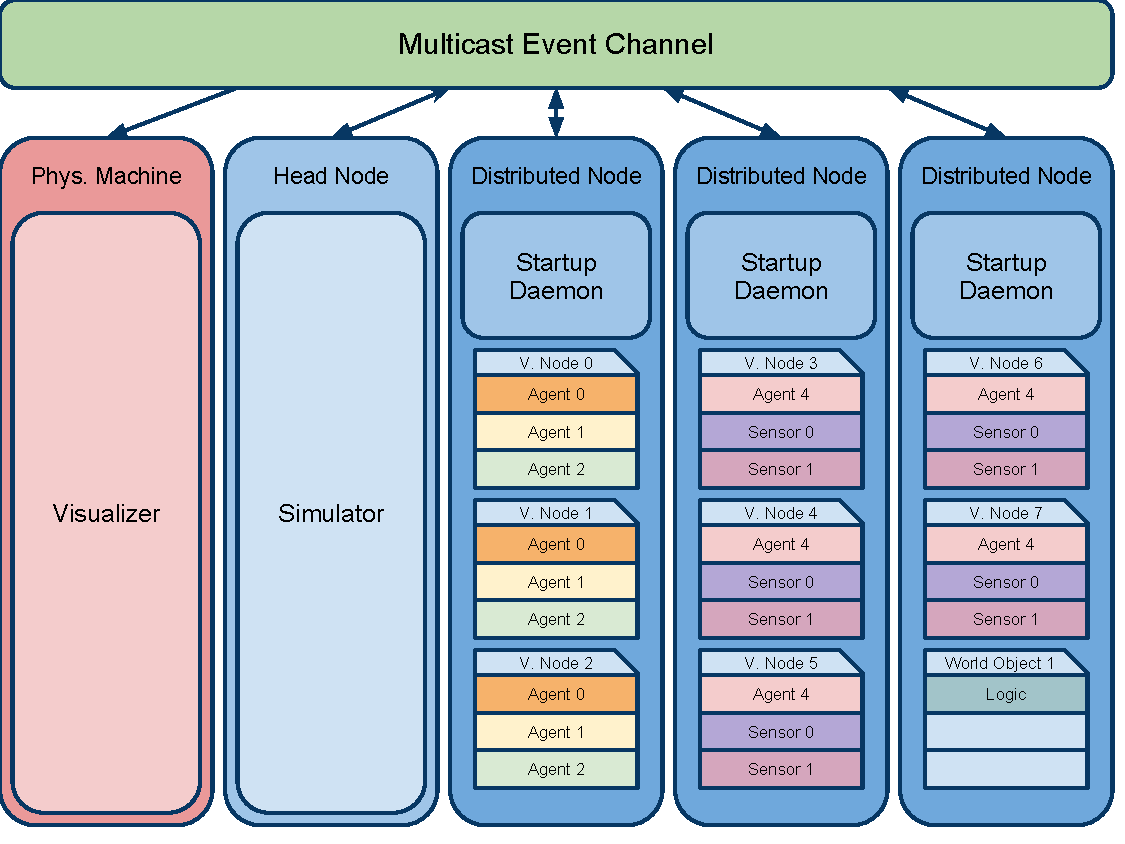
\includegraphics[scale=.6]{../initial-pres/arch.pdf}
    \caption{Distribution Diagram}
    \label{fig-distribution}
\end{figure}
\section{Detailed System Design}
\subsection{Simulator Components}
\subsubsection{Simulation}
\subsubsection{StartupDaemon}
\subsubsection{Entity}
\subsubsection{Built-in Entities}
\paragraph{Node}
\paragraph{PreScriptedObject}
\subsubsection{World}

\subsection{Networking Components}
\subsubsection{Interface}
\subsubsection{CommsEngine}
\subsubsection{Built-in CommsEngines}
\paragraph{LogLossCommsEngine}
\paragraph{EthernetCommsEngine}

\subsection{Event Components}
\subsubsection{Event}
\subsubsection{Built-in Events}
\paragraph{LinkEvent}
\paragraph{CommunicationSendEvent}
\paragraph{EntityMoveEvent}
\paragraph{StartupEvent}
\paragraph{AckStartupEvent}
\paragraph{StartSimulationEvent}
\paragraph{StopSimulationEvent}

\subsection{Agent Components}
\subsubsection{Agent}
\subsubsection{Condition}
\subsubsection{Action}
\subsubsection{Built-in Actions}
\paragraph{Move}

\subsection{Sensor Components}
\subsubsection{Sensor}

\subsection{Utility Components}
\subsubsection{Geo}
\end{document}
